\documentclass[a4paper]{article}

\usepackage{amsmath}
\usepackage{unicode-math}
\usepackage{float}
\usepackage{caption, subcaption}
\usepackage{geometry}
\usepackage{graphicx}
\usepackage{titlesec}
\usepackage{indentfirst}
\usepackage{hyperref}
\usepackage{listings}
\usepackage{xcolor}
\usepackage[lighttt]{lmodern}
\graphicspath{{./images/}}
\geometry{left=20mm,
          right=10mm,
          top=20mm,
          bottom=20mm}


\usepackage{fontspec}
\setmonofont[
  Contextuals={Alternate},
  Scale=MatchLowercase
]{Fira Mono for Powerline}
\lstdefinestyle{bash}{
    basicstyle=\ttfamily,
    framerule=10pt,
    breakatwhitespace=false,
    breaklines=true,
    captionpos=b,
    keepspaces=true,
    showspaces=false,
    showstringspaces=false,
    showtabs=false,
    tabsize=2
}

\lstset{style=bash}
\setmathfont{Latin Modern Math}

\DeclareSymbolFont{cyrletters}{\encodingdefault}{\familydefault}{m}{it}
\newcommand{\makecyrmathletter}[1]{%
\begingroup\lccode`a=#1\lowercase{\endgroup
\Umathcode`a}="0 \csname symcyrletters\endcsname\space #1
}
\count255="409
\loop\ifnum\count255<"44F
\advance\count255 by 1
\makecyrmathletter{\count255}
\repeat

\definecolor{mygray}{rgb}{0.3,0.3,0.3}

\let\oldtexttt\texttt
\renewcommand{\texttt}[1]{\textcolor{mygray}{\oldtexttt{#1}}}


\renewcommand{\thefigure}{\arabic{figure}}
\renewcommand{\theequation}{\arabic{figure}}
\renewcommand{\labelenumii}{\theenumii}
\renewcommand{\theenumii}{\theenumi.\arabic{enumii}.}

\date{\today}

\title{MIPSfpga++ \\ Install Linux on Softcore MIPS on DE10-Lite FPGA. \\ Or just watch me do it. Whatever.}
\author{mmskv}
\date{}

\begin{document}

\pagenumbering{roman}
\maketitle
\tableofcontents

\pagebreak

\pagenumbering{arabic}

\section{Glossary}
\begin{itemize}
    \itemsep0em
    \item \textbf{FPGA} -- Field-Programmable Gate Array, a flexible and customizable hardware platform for implementing digital logic circuits.
    \item \textbf{Softcore CPU} -- Processor core that can be synthesized and implemented on programmable logic devices like FPGAs.
    \item \textbf{MIPSfpga} -- A soft-core MIPS processor provided by Imagination Technologies under a free as in beer license.
    \item \textbf{mipsfpga-plus} -- An Open Source project that introduces UART and SDRAM pin definition to some FPGA boards.
    \item \textbf{BusyBox} -- A set of Unix utilities that have been bundled into a single executable.
    \item \textbf{OpenOCD} -- Open On-Chip Debugger, a software tool that provides debugging, in-system programming, and boundary-scan testing for embedded devices.
\end{itemize}

\section{Prerequisites}
\begin{itemize}
    \itemsep0em
    \item DE10-Lite board
    \item A modern Linux distribution
    \item USB to UART bridge
    \item FT2232 Adapter for OpenOCD with MPSSE support
    \item Serial terminal emulator (minicom is optional)
    \item Docker (Optional)
\end{itemize}

\subsection{Setting up Intel Quartus Prime Lite}

Locate the latest version of Intel Quartus Prime Lite on intel.com and download it. Upon installation, include the Quartus binaries path in our system's PATH.

\subsection{Getting GCC toolchains}

To compile MIPS executables, a specific toolchain is required. Compiling this
toolchain is complex and outside the scope of this document. Therefore, a
Docker image containing a pre-configured toolchain with debugger is provided
for immediate use.

\begin{lstlisting}
    docker pull mmskv/mipsel-linux-gnu-gcc:latest
\end{lstlisting}

\section{Launching MIPS processor on Intel DE10-Lite}

To begin, clone the MIPSfpga-plus repository from GitHub.

\begin{lstlisting}
    git clone https://github.com/MIPSfpga/mipsfpga-plus
\end{lstlisting}

For the MIPSfpga sources, obtain the MIPSfpga Getting Started package (MFGS) that comes with Verilog sources. As the package is not freely distributable, it can't be shared publicly.

Once we have acquired the package, its contents need to be moved into the \texttt{mipsfpga-plus/core} directory.

\begin{lstlisting}
    cp -r MIPSfpga/MIPSfpga_GSG/rtl_up/core/* mipsfpga-plus/core
    cd boards/de10_lite
    make project
    make all # Compiles the project in console with quartus_pgm
\end{lstlisting}

After the Verilog core is compiled, connect the DE10-Lite to the computer using a USB cable to upload the program.

Upload the compiled project via a USB Blaster onto a DE10-Lite.

\begin{lstlisting}
    make load
\end{lstlisting}

We can alternatively use the Quartus GUI instead of Makefiles to achieve the same results.

Optionally open the project in Quartus.

\begin{lstlisting}
    make open
\end{lstlisting}

Once the softcore processor is uploaded to the board, it should start
displaying two counters: one in hexadecimal and one in binary. The \texttt{KEY0} can be
used to reset the counters.

\begin{figure}[H]
    \centering
    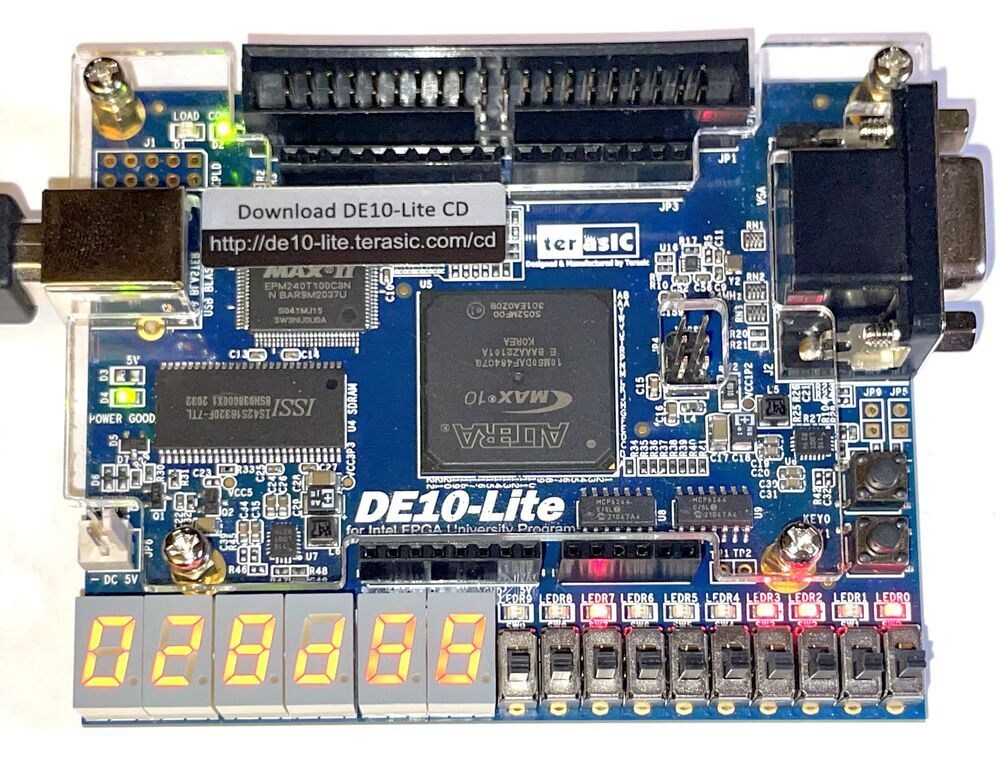
\includegraphics[width=0.5\textwidth]{counter.jpg}
    \captionsetup{width=0.8\textwidth}
    \caption{Counters on the board after mipsfpga load}
\end{figure}

\subsection{Attaching Bus Blaster to Linux (udev)}

Potential error may occur while running the `make load` command

\begin{lstlisting}
    Error (213013): Programming hardware cable not detected
    make: *** [Makefile:38: load] Error 3
\end{lstlisting}

We can diagnose issue with
\begin{lstlisting}
    quartus_pgm --auto
\end{lstlisting}

The error "\texttt{Unable to lock chain - Insufficient port permissions}" indicates
that our user does not have permission to access the Bus Blaster device.
To resolve this, either add the user to the \texttt{usb} group and log back in

\begin{lstlisting}
    sudo usermod -aG usb $(whoami)
\end{lstlisting}

Or set device permissions

\begin{lstlisting}
    sudo dmesg | grep -A5 "USB device number"
    sudo chmod 666 /dev/bus/usb/001/00y # y is the device number
\end{lstlisting}

\subsection{Testing SDRAM}

To test the SDRAM functionality on the softcore processor, use the programs
provided with mipsfpga-plus \cite{mipsfpga_sdram}. One such program is memtest.

\begin{lstlisting}
    cd mipsfpga-plus/programs/06_memtest
\end{lstlisting}

This program was written with support only for a specific archaic MIPS GCC toolchain once distributed by Imagination Technologies.
We can get this toolchain in Docker at \href{https://hub.docker.com/repository/docker/mmskv/mips-mti-elf/general}{mips-mti-elf}.

To compile binary and generate \href{https://en.wikipedia.org/wiki/SREC_(file_format)}{Motorola S-record file} do

\begin{lstlisting}
    docker run -it -v $(pwd):/mipsfpga-plus \
        -w /mipsfpga-plus/programs/06_memtest \
        mmskv/mips-mti-elf:latest \
        make all
\end{lstlisting}

To upload the binary to the CPU, a USB to UART bridge is necessary. UART RX and
TX pin definitions can be set in Quartus 'Pin Planner' or in
\texttt{mipsfpga-plus/boards/de10\_lite/de10\_lite.v}.

Connect USB to UART Adapter:

\begin{itemize}
    \itemsep0em
    \item GPIO 31 -- RX
    \item GPIO 32 -- TX
\end{itemize}

\begin{figure}[H]
    \centering
    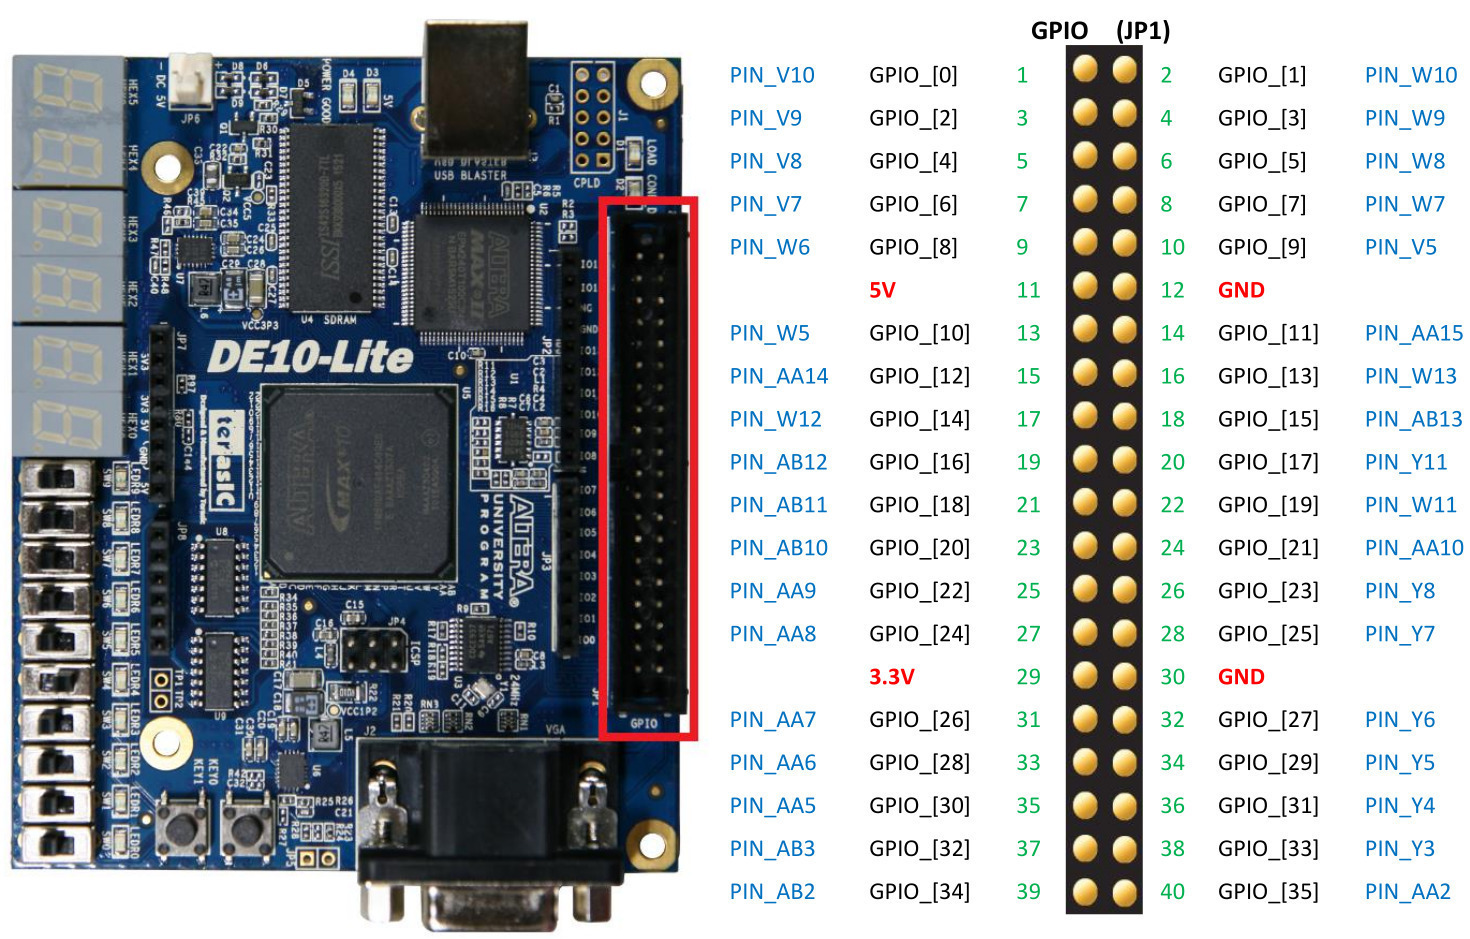
\includegraphics[width=0.8\textwidth]{de10lite-pinout.jpg}
    \captionsetup{width=0.8\textwidth}
    \caption{DE10-Lite I/O pinout.}
\end{figure}

\begin{figure}[H]
    \centering
    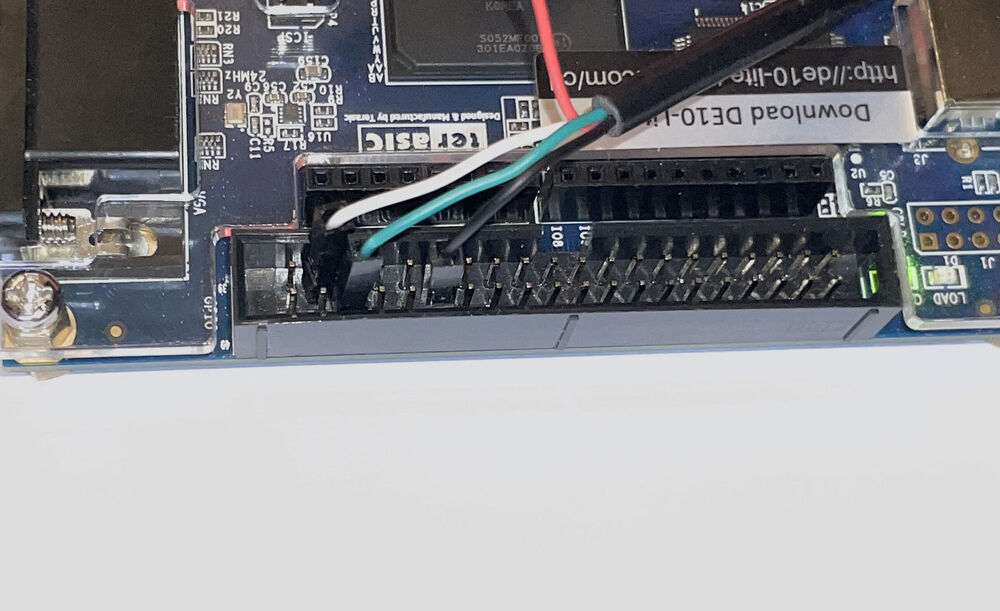
\includegraphics[width=0.5\textwidth]{uart-connection.jpg}
    \captionsetup{width=0.8\textwidth}
    \caption{Correct UART connection.}
\end{figure}

It may be necessary to add our user to the \texttt{dialout} group to access the UART devices as a non-root user

\begin{lstlisting}
    sudo usermod -aG dialout $(whoami)
\end{lstlisting}

Or we can simply set the UART adapter's attributes to \texttt{-rw-rw-rw-}

\begin{lstlisting}
    sudo chmod 666 /dev/ttyUSB0
\end{lstlisting}

Load the instructions onto the CPU. A 5KB binary file transfer should take less
than a second at a 115200bps baud rate. If any hangups occur, try swapping the
RX and TX pin connections.

\begin{lstlisting}
    bash 10_upload_to_the_board_using_uart.sh
\end{lstlisting}

During operation, the LEDs will indicate the current check stage:

\begin{itemize}
    \itemsep0em
    \item LED0 -- Write cycle
    \item LED1 -- Cache reset cycle
    \item LED2 -- Pause
    \item LED3 -- Read cycle
    \item LED4 -- All checks completed, no errors
    \item LED5 -- Errors detected during the checks
\end{itemize}

The 7-segment displays will indicate: two most significant digits -- test
number, four least significant digits -- number of detected read errors.

After approximately 17 minutes, the test should complete and display a result.

\begin{figure}[H]
    \centering
    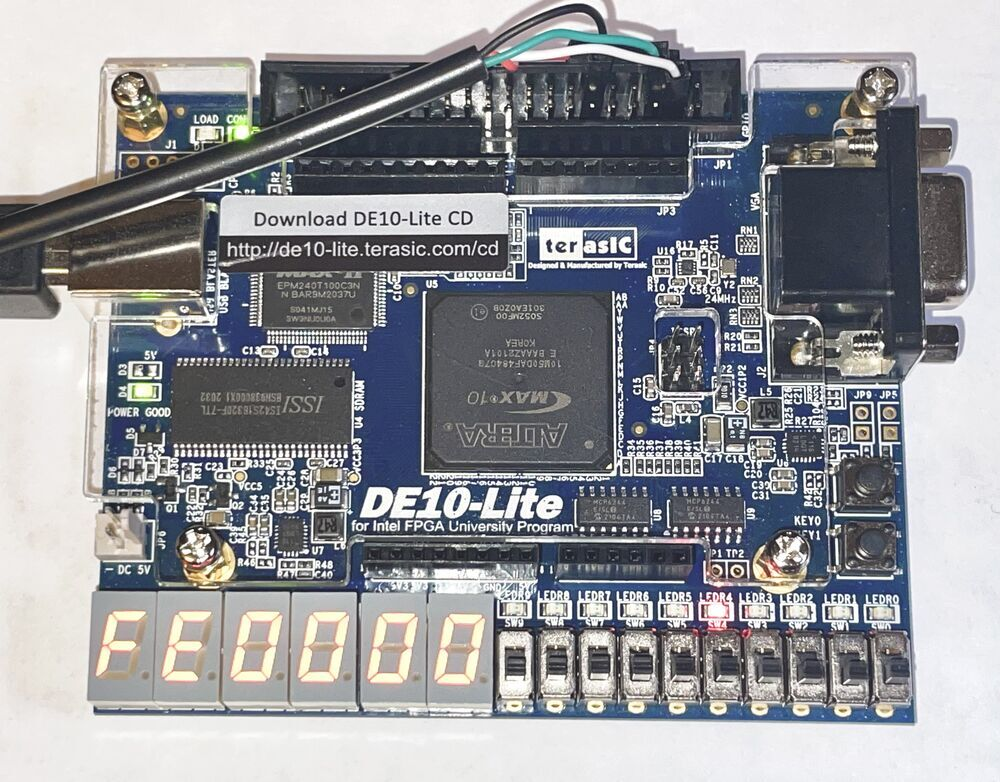
\includegraphics[width=0.5\textwidth]{sdram-test.jpg}
    \captionsetup{width=0.8\textwidth}
    \caption{Successful SDRAM test. Lit LEDR4 means that all checks have passed. 0xFE is the test count and 0x0000 is the error count.}
\end{figure}

\section{Running Linux}

After validating that the SDRAM is functioning correctly, we can proceed with the objective of running Linux.

\subsection{Building BusyBox initramfs}

Since the DE10-Lite lacks built-in storage, we'll utilize filesystem in RAM
images. BusyBox is an ideal option for this task due to its compact size -
about 1MB of our 32MB SDRAM. Although GNU could potentially fit after some
modifications, we'll proceed with BusyBox for simplicity.

\begin{lstlisting}
    git clone https://github.com/buildroot/buildroot --depth 1
    cd buildroot
    wget https://raw.githubusercontent.com/mmskv/mipsfpga-plusplus/master/patches/buildroot.patch
    git apply patch
    make de10lite_defconfig
    make -j $(nproc)
\end{lstlisting}

Now we should have a rootfs.cpio at \texttt{./output/images/}. We will use it later.

\subsection{Building Linux}

Get the sources

\begin{lstlisting}
    git clone https://github.com/torvalds/linux --depth 1
    cd linux
\end{lstlisting}

As noted in article \cite{mipsfpga_linux}, the modified
\texttt{arch/mips/xlifpga} was used to build Linux for MIPSfpga. Unfortunately,
this target since was removed in the commit
\href{https://github.com/torvalds/linux/commit/0861aa1251c749bbec4ee124ee21660c2f263da4}{0861aa1251c749bbec4ee124ee21660c2f263da4}.
Reverting this commit won't work due to numerous subsequent changes. However, a
patch that introduces MIPSfpga++ as a platform can be applied to the Linux tree

\begin{lstlisting}
    wget https://raw.githubusercontent.com/mmskv/mipsfpga-plusplus/master/patches/linux.patch
    git apply
\end{lstlisting}

With the \texttt{arch/mips/mipsfpga-plusplus} target added, Linux can now be built.

Generate \texttt{.config}

\begin{lstlisting}
    make ARCH=mips BOARDS=mipsfpga-plusplus 32r2el_defconfig
\end{lstlisting}

Path to the initramfs image has to be specified either with a single command or with menuconfig

\begin{lstlisting}
    ./scripts/config --set-val INITRAMFS_SOURCE \"/path/to/buildroot/output/images/rootfs.cpio\"
    # or with menuconfig
    make MENUCONFIG_COLOR=blackbg ARCH=mips menuconfig
\end{lstlisting}

When compiling the kernel a MIPS toolchain has to be specified since we are
building for a non native target. For easier dependency management we will do
it in a Docker container that has a MIPS toolchain and multiarch gdb.

\begin{lstlisting}
    docker run \
        --network=host -it \
        -v $(pwd)/..:/workdir \
        -w /workdir/linux \
        mmskv/mipsel-linux-gnu-gcc:latest \
        make -j $(nproc) ARCH=mips CROSS_COMPILE=/usr/sbin/mips64el-linux-gnu-
\end{lstlisting}

\subsection{Loading linux}

OpenOCD is added by mipsfpga-plus for loading and debugging programs running on the CPU.

Connect FT2232 to the board as follows:

\begin{itemize}
    \itemsep0em
    \item GPIO 17 -- TCK
    \item GPIO 19 -- TDO
    \item GPIO 21 -- TDI
    \item GPIO 23 -- TMS
\end{itemize}

Connect UART dongle:

\begin{itemize}
    \itemsep0em
    \item GPIO 33 -- TX
    \item GPIO 35 -- RX
\end{itemize}

\begin{figure}[H]
    \centering
    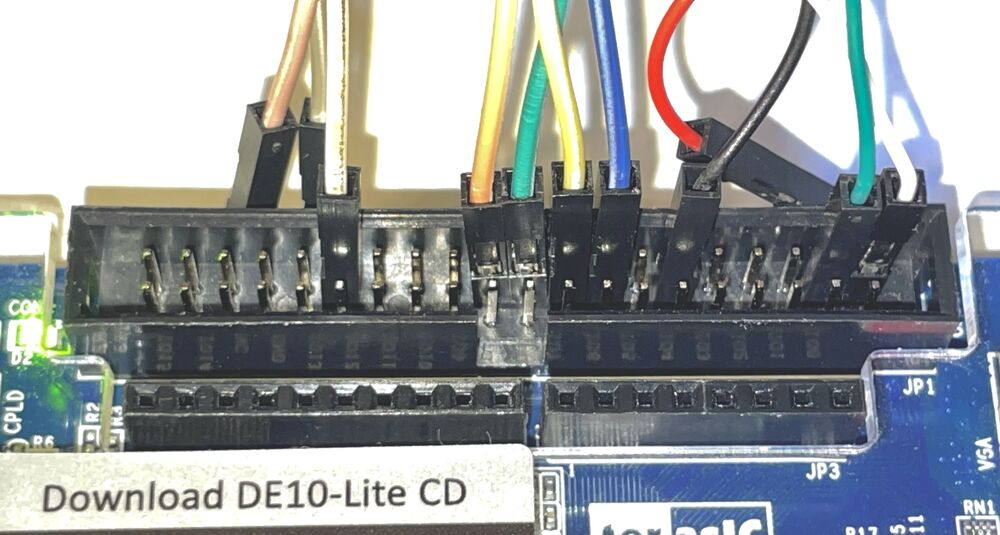
\includegraphics[width=0.5\textwidth]{uart-jtag.jpg}
    \captionsetup{width=0.8\textwidth}
    \caption{JTAG and UART connection.}
\end{figure}

Start OpenOCD. The OpenOCD configuration is board specific.

\begin{lstlisting}
    openocd -f <ft2232 config>.cfg
\end{lstlisting}

We can then use gdb to load the Linux binary onto the CPU. Note that there are
two files in the current diretory; vmlinux is a binary with debug symbols,
while vmlinuz is a binary with stripped debug symbols.

GDB has to be specifically compiled with MIPS target support so we will use custom gdb in a Docker container

\begin{lstlisting}
    docker run \
        --network=host -it \
        -v $(pwd):/linux \
        -w /linux \
        mmskv/mipsel-linux-gnu-gcc:latest \
        gdb-multiarch vmlinux
\end{lstlisting}

Upon seeing the gdb shell, connect to the openocd gdb port (default: 3333)

\begin{lstlisting}
    (gdb) target extended-remote :3333
\end{lstlisting}

Load the Linux binary (this will take around 5 minutes)

\begin{lstlisting}
    (gdb) load
\end{lstlisting}

At this point, we can execute the loaded kernel

\begin{lstlisting}
    (gdb) continue
\end{lstlisting}

The kernel will use the UART interface as a virtual console. If the kernel ring
buffer logs don't appear after 5 seconds, consider swapping the RX and TX UART
pins. After approximately 30 more seconds, the following login prompt should appear

\begin{lstlisting}
    Welcome to MIPSfpga++
    mipsfpga-plusplus login:
\end{lstlisting}

Now, we can log in as \texttt{root} and start exploring our Linux environment on the softcore MIPS processor.

\subsection{Running a program on Linux on MIPS on FPGA}

In this section, we'll be going through the steps to execute a simple "Hello
World" program on our MIPS softcore CPU.

One of the most challenging aspects of this task is transferring our compiled
binary into the board's filesystem. The reason for this challenge is due to the
fact that our only interface with the system is through a serial connection.

Let's begin by creating a C source file named \texttt{helloworld.c}:

\begin{lstlisting}
    #include <stdio.h>

    int main(void){
        puts("Hello world\n");
        return 0;
    }
\end{lstlisting}

Once you've created the source file, compile it using the following command:

\begin{lstlisting}
    docker run -it -v $(pwd):/workdir \
        -w /workdir/ \
        mmskv/mipsel-linux-gnu-gcc:latest \
        mips64el-linux-gnu-gcc -LE -march=24kc -mabi=32 helloworld.c -o helloworld
\end{lstlisting}

Upon successful compilation, you'll obtain the binary file `helloworld`. To
transfer this binary to our system, we'll need to encode it into a format that
can be safely transferred over a serial connection. Here's where the command
\texttt{cat helloworld | xz | base64} comes into play.

This command performs the following operations:

\begin{enumerate}
    \itemsep0em
    \item '\texttt{cat helloworld}': This reads the binary file and sends its
        contents to the standard output.
    \item '\texttt{| xz}': The pipe symbol (\texttt{|}) redirects the output from
        the preceding command into the \texttt{xz} command, which compresses
        the binary data. This reduces the size of the data that needs to be
        transferred because it has many empty regions.
    \item '\texttt{| base64}': This again redirects the output -- this time, the
        compressed data -- into the \texttt{base64} command. Base64 encoding is
        used to convert binary data into a text format, making it safe for
        transfer over protocols that are designed to handle text, in our case
        the serial tty.
\end{enumerate}

The output of this command is a base64-encoded string representing the
compressed binary. This can be selected and pasted into the Linux serial
console.

However, a direct paste operation with heredocs might not be successful,
because the CPU's processing speed might not keep up with the paste speed
(noticeable from \texttt{ttyS ttyS0: 87 input overrun(s)} messages in the
kernel logs). To circumvent this, a paste delay needs to be added in Minicom.

\begin{lstlisting}
    cat helloworld | xz | base64
\end{lstlisting}

Select resulting base64 to then paste it in Linux serial console

Simply pasting the stuff with heredocs won't work, because the cpu is so slow
it can't read characters at the paste speed. (look for '\texttt{ttyS ttyS0: 87 input
overrun(s)'} messages in kernel logs).

Start \texttt{minicom} terminal

\begin{lstlisting}
    minicom -b 115200 -D /dev/ttyUSB0
\end{lstlisting}

Add a paste delay with the following key presses

\begin{lstlisting}
    Ctrl-A, Z, O, Serial Port Setup, F, <Esc>, <Esc>
    Ctrl-A, Z, T, F, <Basckspace>, 1, <Esc>, <Esc>
\end{lstlisting}

Next, we'll decode and decompress the binary, set the correct permissions, and finally run it

\begin{lstlisting}
    cat <<EOF | base64 -d | unxz > helloworld
    <Ctrl-Shift-V to paste your base64 encoded binary>
    EOF

    chmod +x helloworld
    ./helloworld
\end{lstlisting}

\begin{figure}[H]
    \centering
    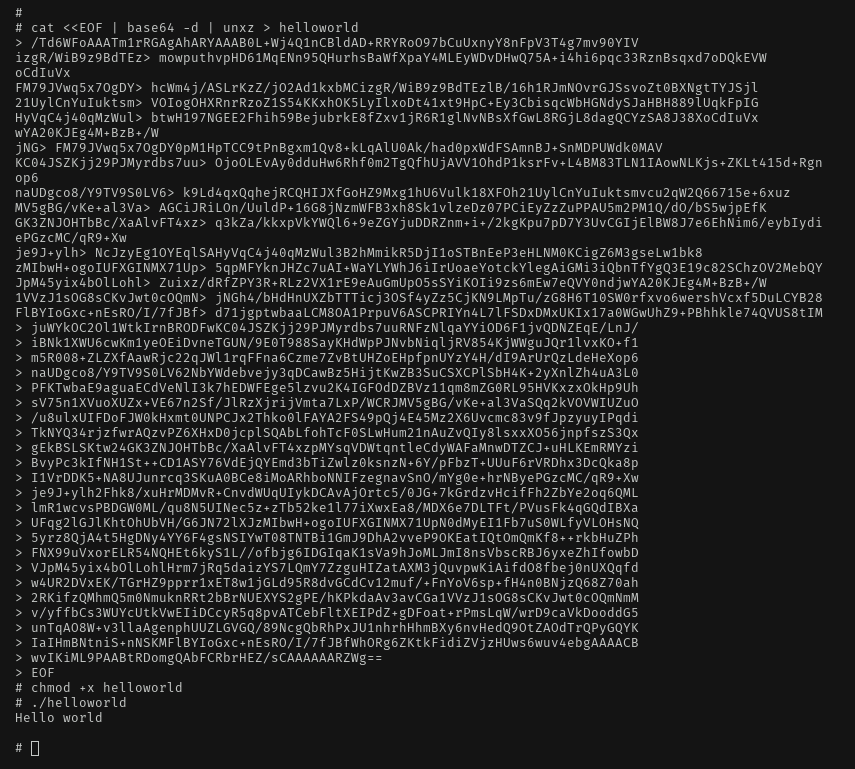
\includegraphics[width=0.7\textwidth]{helloworld.png}
    \captionsetup{width=0.8\textwidth}
    \caption{Sending a helloworld binary and running it.}
\end{figure}


For those unfamiliar, the \texttt{<<EOF} syntax is known as a "here document"
or "heredoc". It's a way of providing a block of text (possibly including shell
script) as input to a command. This is typically used in shell scripting for
multi-line input to a command. More information on heredocs can be found in the
\href{https://en.wikipedia.org/wiki/Here_document}{Wikipedia}.

\section{Discussion and future work}

The current Linux configuration implemented in this project, while functional,
is not necessarily optimal. There is room for further refinement to enhance the
performance and security of the system. The .config file contains many options
that could potentially be disabled to create a lighter, faster, and more secure
Linux image.

During the project, it was observed that the board occasionally encountered
memory errors through the JTAG interface. This issue resulted in system
instability, causing the board to fail unexpectedly. The current workaround
for this issue is to reflash the board using Quartus.

Another area that needs attention is the General Purpose Input/Output (GPIO)
system. In this project, the GPIO functionality has not been extensively
tested.

\pagebreak

\begin{thebibliography}{99}

\bibitem{mipsfpga_sdram}
Stanislav Zhelnio,
\textit{MIPSfpga and SDRAM},
Habr,
2017,\\
\url{https://habr.com/en/articles/321530/},

\bibitem{mipsfpga_linux}
Stanislav Zhelnio,
\textit{Running Linux on MIPSfpga and Altera FPGA},
Habr,
2017,\\
\url{https://habr.com/en/articles/333920/},

\end{thebibliography}

\end{document}

